\section{Бесперапынная інтэграцыя і дастаўка}

\subsection{Асноўныя паняцці}

Бесперапынная інтэграцыя азначае, што зборка і тэсціраванне (Unit-testing)
праграмнага забеспячэння адбываюцца аўтаматычна і часта.
Частата азначае, зборка праграмнага забеспячэння адбываецца перыядычна
альбо, напрыклад, пры кожным змяненні ў кантролі версій змяненняў.
Заўважым, што ключавым момантам ў бесперапыннай інтэграцыі з'яўляецца тое,
што працэс тэсціравання (інтэграцыя праграмнага забеспячэння) аўтаматызаваны
пры дапамозе інструментаў і не патрабуе ручнога ўмяшання падчас
зборкі і тэсціравання%
[\ref{book:Continuous Integration}].

Бесперапынная дастаўка азначае, што праграмнае забеспячэнне
заўсёды гатовае да разгортвання.
Праграмнае забеспячэнне збіраецца і тэсціруецца падчас працэсаў
бесперапыннай інтэграцыі і, таксама, разгортваецца ў адмысловае
асяроддзе для далейшых тэстаў.
Ключавым момантаў у бесперапыннай дастаўцы з'яўляецца тое,
што кожная версія зборкі аўтаматычна правяраецца на гатоўнасць да
разгортвання[\ref{book:Continuous Delivery}].

Бесперапыннае разгортванне азначае аўтаматычнае разгортванне
праграмнага забеспячэння ў вытворчасць пасля таго, як
унесены змены ў вытворчую галіну кантроля версіі і паспяхова пройдзены
аўтаматычныя тэсты на праверку гатоўнасці да разгортвання.
Зборка, тэсціраванне, разгортванне ажыццяўляюцца без ўмяшання чалавека%
[\ref{book:Continuous Delivery vs. Continuous Deployment}].

Такім чынам адрозненнем паміж бесперапыннай дастаўкай і разгортваннем
з'яўляецца тое, што пры працэсе бесперапыннай дастаўкі праграмнае
забеспячэнне сцвярджаецца гатовым да разгортвання ў вытворчасць чалавекам.
У той жа час пры працэсе бесперапыннага разгортвання праграмнае
забеспячэнне аўтаматычна разгортваецца ў вытворчасць.

Бесперапынная дастаўка і разгортванне часта памылкова ўжываюцца як
сінонімы, аднак неабходна разумець, што розніца паміж гэтымі двума
тэрмінамі існуе. На малюнку \ref{figure:relations of CI, CD, CD}
прад\-стаў\-ле\-ны ўзаемаадносіны паміж бесперапыннай інтэграцыяй,
дастаўкаў і разгортваннем.

\begin{figure}[h!]
    \centering
    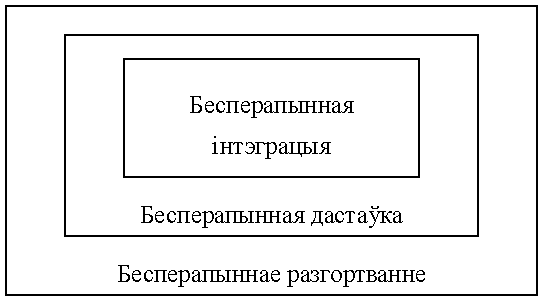
\includegraphics{Relations_of_CI_CD_CD.pdf}
    \caption{Узаемаадносіны паміж бесперапыннай
             інтэграцыяй, дастаўкай і разгортваннем}
    \label{figure:relations of CI, CD, CD}
\end{figure}

Згодна з малюнкам \ref{figure:relations of CI, CD, CD}
можна сцвярджаць, што немагчыма пабудаваць канвеер бесперапыннага
разгортвання без працэсаў бесперапыннай інтэграцыі і дастаўкі,
так як адно ўключае ў сябе другое.

На малюнку \ref{figure:Difference_between_CD_and_CD}
прадстаўлены канвееры бесперапыннай дастаўкі і разгортвання.

\begin{figure}[h!]
    \centering
    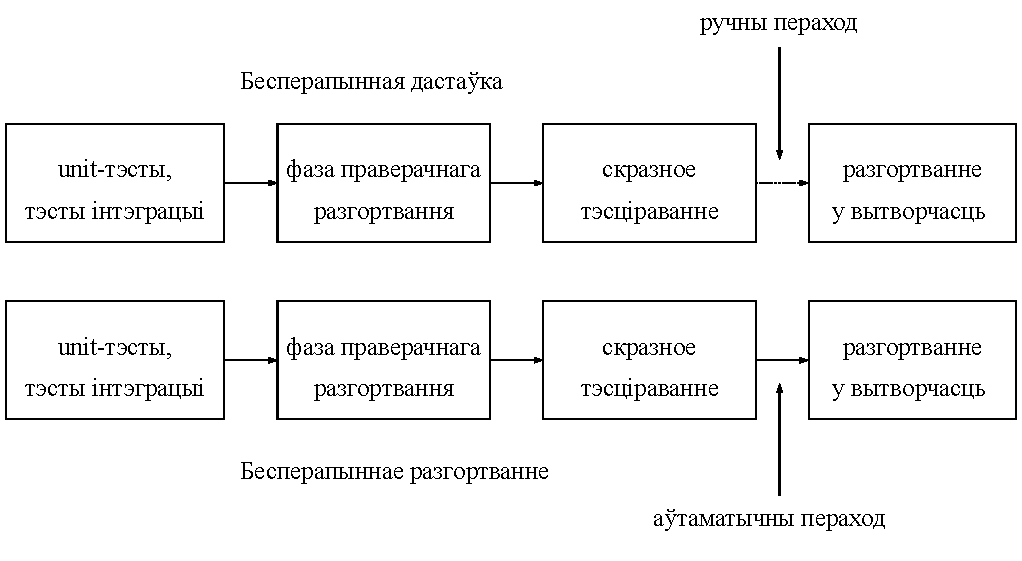
\includegraphics[width=\linewidth]{Difference_between_CD_and_CD.pdf}
    \caption{Адрозненне паміж бесперапыннай дастаўкай і разгортваннем}
    \label{figure:Difference_between_CD_and_CD}
\end{figure}

Падвядзем ітог тэрміналогіі:
\begin{enumerate}
    \item Бесперапынная інтэграцыя -- гэта набор практык,
          мэта каторага паляпшэнне якасці і хуткасці распрацоўкі
          праграмнага забеспячэння пры дапамозе аўтаматызацыі
          зборкі і тэсціравання, а таксама памяншэнне імавернасці
          памылак праз ручную зборку альбо праз розныя
          ўласцівасці асяроддзя выканання зборкі.
          Бесперапынная інтэграцыя з'яўляецца часткай бесперапыннай
          дастаўкі;
    \item Бесперапынная дастаўка -- гэта набор практык,
          які ўключае ў сябе бесперапынную інтэграцыю і дадае 
          да яе аўтаматызацыю скразнога тэсціравання і дастаўку
          праграмнага забеспячэння такім чынам, каб канчатковая
          зборка праграмы магла прымяняцца на патрэбных платформах
          і пры пэўных умовах.
          Бесперапынная дастаўка з'яўляецца часткай бесперапыннага
          разгортвання і не ўключае ў сябе аўтаматычнае
          разгортванне праграмнага забеспячэння ў вытворчасць;
    \item Бесперапыннае разгортванне -- гэта набор практык, які
          ўключае ў сябе вышэй узгаданыя бесперапынную інтэграцыю
          і дастаўку, аднак дадае да іх аўтаматычнае разгортванне
          праграмнага забеспячэння ў вытворчасць.
          Пры ідэальных умовах, канвеер бесперапыннага разгортванне
          не патрабуе чалавечага ўмяшання для абнаўлення альбо выпуску
          новых рэлізаў праг\-рам\-на\-га забеспячэння.
\end{enumerate}

\subsection{Перавагі бесперапыннай інтэграцыі}

Пры ўмове, што ўкараненне бесперапыннай інтэграцыі адбываецца карэктна,
яна прадастаўляе камандзе распрацоўшчыкаў наступныя перавагі%
[\ref{book:Continuous Integration}]:

\begin{enumerate}
    \item памяншэнне рызык;
    \item аўтаматызацыя працэсаў, якія паўтараюцца;
    \item прыдатнасць праграмнага забеспячэння да разгортвання
          дзе заўгодна і калі заўгодна;
    \item лепшая бачнасць праекта;
    \item большая ўпэўненасць каманды ў якасці праграмнага забеспячэння.
\end{enumerate}

Найбольш папулярнай перавагай бесперапыннай інтэграцыі з'яўляецца
памяншэнне рызык. Гэта дасягаецца тым, што інтэграцыя (аб'яднанне
розных частак праграмы) адбываецца некалькі разоў на дзень.
Такая частата інтэграцыі дазваляе распрацоўшчыкам хутка знаходзіць
і выпраўляць памылкі, а таксама адсочваць якасці праграмнага забеспячэння
з меншым інтэрвалам часу. Нарэшце, частая зборка дазваляе атрымліваць
у рэальным часу і дакладную зва\-рот\-ную сувязь пасля кожнай інтэграцыі.

Аўтаматызацыя руцінных задач не меншая перавага ад бесперапыннай
інтэграцыі. Аўтаматызаваныя сістэмы і працэсы захоўваюць час, грошы
і сілы. Такім чынам аўтаматызацыя дазваляе супрацоўнікам сканцэнтравацца
на іншых задачах.

З пункту гледжання кліента, вялікай перавагай з'яўляецца факт таго,
што праграмнае забеспячэнне заўсёды прыдатнае да разгортвання.
Дзякуючы бесперапыннай інтэграцыі праграмнае забеспячэнне можа
быць лёгка абноўлена невялікімі змяненнямі і адразу ж гатоввым да
разгортвання.

Бесперапынная інтэграцыя дазваляе распрацоўшчыкам магчымасць бачыць
стан усяго праекта. Напрыклад, у мінулым для таго, каб прыняць
рашэнне аб абнаўленні, распрацоўшчыку патрабавалася збіраць неабходныя
даныя ўручную альбо толькі рабіць прапановы наконт невядомых даных.
Як вынік, працэс збору інфармацыі займаў шмат часу і энергіі,
і ў той жа час мог не забяспечваць усёй неабходнай інфармацыей.
Аднак дзякуючы ўкараненню практыкі бесперапыннай інтэграцыі,
дадзены працэс стаў нашмат прасцей.
Сістэма прапаноўвае ў рэальным часу інфармацыю пра апошнюю зборку
праграмнага забеспячэння, адсотак памылак і прагрэс завяршэння.

Нарэшце, калі сістэма прапускае праграмнае забеспячэнне
праз серыю аўтаматычных тэстаў і праверак, каманда распрацоўшчыкаў
упэўнена ў якасці праграмы і яе прыдатнасці да разгортвання
пры ўмове, што зборка завяршылася паспяхова.
У адваротным выпадку, сістэма неадкладна інфарміруе распрацоўшчыкаў
аб наяўнасці праблем і іх прычын.

\subsection{Перавагі бесперапыннай дастаўкі}

Адпаведна вышэй напісанаму, што бесперапынная інтэграцыя з'яўляецца
часткай бесперапыннай дастаўкі, вынікае, што бесперапыннай дастаўка
мае ўсе перавагі бесперапыннай інтэграцыі.

Аднак бесперапынная дастаўка прапаноўвае і іншыя перавагі, якія
памяншаюць іма\-вер\-насць узнікнення стрэсавай сітуацыі ў супрацоўнікаў.
Пры дапамозе аўтаматызацыі кожнага ручнога працэса, які неабходна
час ад часу паўтараць, супрацоўнікі пазбягаюць памылак і заўжды
перакананы, што праграмнае забеспячэнне стабільнае, правільна
сканфігураванае і прыдатнае да разгортвання.
Як вынік, дзень рэліза праграмнага забеспячэння праходзіць менш
інтэнсіўна і з меншым стрэсам.
Што, у сувязі з паскоранымі тэмпамі выпуску новых прадуктаў
альбо абнаўленій старых версій праграм, становіцца неабходным складнікам
для падтрымання стабільнага эмацыянальнага становішча ўнутры кампаніі.

Нарэшце, так як працэс выпуску новых рэлізаў становіцца больш гладкім і
стабільным, гэта дазваляе кампаніі хутчэй дастаўляць
праграмнае забеспячэнне кліентам.
Бесперапынная дастаўка развязвае задачу пра неабходнасць
неадкладнай дастаўкі кліентам якасных версій праграмнага забеспячэння
пры дапамозе аўтаматызаваных канфігурацый вытворчага асяроддзя, што
забяспечвае прыдатнасць праграмнага забеспячэння да разгортвання
ў любы час і на любую платформу.


\subsection{Інструменты бесперапыннай інтэграцыі і дастаўкі}

У дадзеным падраздзеле разглядаюцца некаторыя папулярныя інструменты для
рэалізацыі прыцыпаў бесперапыннай інтэграцыі і дастаўкі,
і іх асаблівасці.

\subsubsection{Jenkins}

Jenkins -- найбольш папулярны праект з адкрытым кодам для аўтаматызацыі.
Дадатковае мноства плагінаў Jenkins дазваляе аўтаматызаваць
любую неабходную задачу.
Jenkins выкарыстоўваецца для зборкі праекта, запуску тэстаў,
аналізу кода і разгортвання праекта.

Асаблівасці Jenkins:
\begin{enumerate}
    \item Jenkins можа працаваць як незалежны CI сервер альбо
          як платформа бесперапыннай дастаўкі для любога праекта;
    \item наяўнасць зборак для Unix, Windows і OS X, што
          спрашчае працэс устаноўкі;
    \item наяўнасць Web-інтэрфейса для хуткай канфігурацыі сервера;
    \item разнастайныя плагіны для зборкі і кіравання зыходным кодам,
          задач адміністравання, інтэрфейсу карыстальніка.
\end{enumerate}

\subsubsection{Travis}

Travis CI -- гэта платформа бесперапыннай інтэграцыі для аўтаматызацыі
працэсаў тэсціравання і разгортвання праграмнага забеспячэння.
Travis CI рэалізуецца ў якасці платформы, якая аб'ядноўваецца з
GitHub праектамі, што дазваляе праводзіць тэсціравання кода
ў рэальным часе.

Travis CI прадугледжвае бясплатнае выкарыстанне для адкрытых праектаў і
платная для камерцыйный праектаў.

Асаблівасці Travis CI:
\begin{enumerate}
    \item бясплатная версія для акрытых праектаў на GitHub;
    \item простая рэгістрацыя і дабаўленне праектаў;
    \item аўтаматызаваная праверка pull-запытаў;
    \item багатая падтрымка паведамленняў
          (напрыклад, e-mail, Slack, HipChat);
    \item наяўнасць API і кансольных інструментаў для
          гібкай настройкі.
\end{enumerate}

\subsubsection{GitLab CI}

GitLab -- хуткаразвіваемая платформа для кіравання коду.
GitLab прапаноўвае ў межах адзінай панелі
інструменты для кіравання рэлізаў,
прагляду коду, бесперапыннай інтэграцыі і разгортвання.

GitLab прадугледжвае бясплатнае выкарыстанне для адкрытых праектаў і
платная для камерцыйный праектаў.

Асаблівасці GitLab CI:
\begin{enumerate}
    \item наяўнасць зборак для папулярных версій Linux;
    \item прыязны інтэрфейс карыстальніка;
    \item падрабязная дакументацыя для кожнай функцыі;
    \item магчымасць індывідуальнай настройкі тэстаў
          для кожнай галіны праекта;
    \item ручное разгортванне і лёгкай магчымасць вяртання
          на папярэднію версію.
\end{enumerate}

\subsubsection{Chef}

Chef забяспечвае асяроддзе для аўтаматызацыі кіравання
інфраструктурай, разгортваннем, канфігурацыяй незалежна
ад памераў сеткі. Chef можна лёгка інтэгравацца ў
воблачныя сервісы, фізічныя серверы альбо гібрыдныя рашэнні.

Асаблівасці Chef:
\begin{enumerate}
    \item убудаваныя наборы інструментаў для аўтаматызацыі
          інфраструктуры як код;
    \item магчымасць кіравання як воблачнымі, так і фізічнымі
          серверамі;
    \item лёгкі перавод праграмы паміж воблачнымі серверамі.
\end{enumerate}

\subsubsection{Puppet}

Платформа Puppet выкарыстоўваецца для кіравання канфігурацыяй для
Unix і Windows сістэмы.
Puppet -- інструмент кіравання канфігурацыяй з адкрытым кодам.
Puppet дазваляе распрацоўшчыкам дастаўляць і выкарыстоўваць
праграмнае забеспячэнне незалежна ад яго крыніцы.

GitLab прадугледжвае бясплатны тэрмін выкарыстання для азнакамлення.

Асаблівасці Puppet:
\begin{enumerate}
    \item наяўнасць гібкай настройкі Puppet-агента і кансолей, што
          дазваляе аб'ядноўваць працэсы бесперапыннай інтэграцыі;
    \item наяўнасць бясплатных модулей для хуткай распрацоўкі;
    \item прадугледжваецца сумесная работа з Git і Jenkins для
          бесперапыннай аўтаматызацыі.
\end{enumerate}

\subsubsection{Better Code Hub}

Better Code Hub -- Web-сервіс для аналізу зыходнага кода.

Better Code Hub прадугледжвае бясплатнае выкарыстанне
для адкрытых праектаў і платная для камерцыйный праектаў.

Асаблівасці Better Code Hub:
\begin{enumerate}
    \item неадкладная зваротная сувязь на кожнае змяненне кода;
    \item інтэграцыя з GitHub;
    \item гібкая настройка прыярытэтаў дзеянняў.
\end{enumerate}

\subsubsection{Docker}

Docker -- праграмнае забеспячэнне для аўтаматызацыі разгортвання і
кіравання праграмамі ў асяроддзі з падтрымкай кантэйнерызацыі.
Docker дазваляе ўпакаваць праграму з неабходным асяроддзем і
залежнасцямі ў кантэйнер, які можа быць перанесены на любую
Linux-сістэму.

Асаблівасці Docker:
\begin{enumerate}
    \item незалежнасць праграмы ад сістэмы, на якой выконваецца
          запуск;
    \item павялічаная бяспека сістэмы;
    \item лёгкая дастаўка праграмнага забеспячэння кліенту.
\end{enumerate}
